\documentclass{../common/SCNU_Experimental_Report}

% 填写报告头信息
\studentname{汤承洲}
\studentid{20233902058}
\major{电子信息工程}
\class{23级2班}
\coursename{控制工程}
\projectname{控制系统现代分析}
\verify
\experimentdate{2026年6月2日}
\teacher{熊爱民}

\graphicspath{{./figures/}}

\begin{document}
\maketitle

\section{实验目的}
\begin{enumerate}
    \item 掌握如何使用MATLAB进行系统的稳定性分析，包括代数法（Routh判据、求特征根）和频域法（Bode图）两种方法。
    \item 掌握如何使用MATLAB进行系统的能控性、能观性分析，包括能控性矩阵、能观性矩阵以及Gramian矩阵方法。
    \item 掌握如何使用MATLAB进行离散系统分析，研究不同采样率对离散化精度的影响。
\end{enumerate}

\section{实验原理}
\subsection{系统稳定性分析原理}
控制系统稳定性的判定是控制理论的核心问题之一。本实验采用代数法和频域法两种方法进行稳定性分析。

\textbf{代数法稳定性判据：}通过求解闭环特征方程的根来判断系统稳定性。若所有特征根均具有负实部（位于左半s平面），则系统稳定。Routh-Hurwitz判据通过构造Routh表，检查第一列系数的符号变化次数，判断特征根中位于右半s平面的个数，无需直接求解特征方程。

\textbf{Bode图法稳定性判据：}基于Nyquist稳定判据，通过开环系统的频率响应特性判断闭环稳定性。幅值裕度（Gain Margin）和相角裕度（Phase Margin）是衡量系统相对稳定性的重要指标。对于最小相位系统，当幅值裕度$>0$~dB且相角裕度$>0^\circ$时，闭环系统稳定。

\subsection{系统能控性与能观性分析原理}
\textbf{能控性（Controllability）：}若存在一个无约束的控制向量$\boldsymbol{u}(t)$，能在有限时间$[t_0, t_f]$内将系统从任意初始状态$\boldsymbol{x}(t_0)$转移到任意终态$\boldsymbol{x}(t_f)$，则称系统状态完全能控。能控性判据为能控性矩阵$\boldsymbol{C}_o = [\boldsymbol{B}, \boldsymbol{AB}, \boldsymbol{A}^2\boldsymbol{B}, \ldots, \boldsymbol{A}^{n-1}\boldsymbol{B}]$满秩（$\text{rank}(\boldsymbol{C}_o) = n$）。

\textbf{能观性（Observability）：}若在有限时间$[t_0, t_f]$内，通过测量输出$\boldsymbol{y}(t)$能唯一确定系统的初始状态$\boldsymbol{x}(t_0)$，则称系统状态完全能观。能观性判据为能观性矩阵$\boldsymbol{O}_b = [\boldsymbol{C}, \boldsymbol{CA}, \boldsymbol{CA}^2, \ldots, \boldsymbol{CA}^{n-1}]^\mathrm{T}$满秩（$\text{rank}(\boldsymbol{O}_b) = n$）。

对于稳定系统，还可以通过求解Lyapunov方程得到能控性Gramian矩阵$\boldsymbol{W}_c$和能观性Gramian矩阵$\boldsymbol{W}_o$，其秩同样可用于判断能控性和能观性。

\subsection{采样率影响分析原理}
数字控制系统需要对连续信号进行采样和离散化。根据香农采样定理，采样频率$f_s$必须大于信号最高频率的两倍（即$f_s > 2f_{\max}$），才能从采样信号中无失真地恢复原始信号。本实验通过零阶保持器（ZOH）方法将连续系统离散化，在不同采样率下比较离散系统与连续系统的频率响应差异，分析采样率对离散化精度的影响。

\section{实验内容}
\subsection{Task 01：系统稳定性分析}

\subsubsection{代数法稳定性判据}
已知系统的开环传递函数为：
\[
G(s) = 100\frac{s + 3}{s(s + 1)(s + 10)}
\]
对系统闭环判别其稳定性。闭环特征多项式为：
\[
1 + G(s) = 0 \quad \Longrightarrow \quad s(s+1)(s+10) + 100(s+3) = 0
\]
展开得：
\[
s^3 + 11s^2 + 110s + 300 = 0
\]

\textbf{方法一：求特征根。}求解闭环特征多项式，得到特征根：
\begin{itemize}
    \item $-3.7007 + 8.3469i$
    \item $-3.7007 - 8.3469i$
    \item $-3.5986$
\end{itemize}
三个根均具有负实部，全部位于左半s平面，故闭环系统稳定。

\textbf{方法二：Routh判据。}构造Routh表如下：
\[
\begin{array}{c|cc}
s^3 & 1 & 110 \\
s^2 & 11 & 300 \\
s^1 & 82.7273 & 0 \\
s^0 & 300 & 0
\end{array}
\]
Routh表第一列系数为：1、11、82.7273、300，全部为正数，无符号变化，故闭环系统稳定。两种方法结论一致。

\subsubsection{Bode图法判断系统稳定性}
已知两个单位负反馈系统的开环传递函数分别为：
\[
G_1(s) = \frac{3}{s^3 + 5s^2 + 3s},\qquad
G_2(s) = \frac{3}{s^3 + 5s^2 - 3s}
\]
用Bode图法判断系统闭环的稳定性。

\begin{figure}[H]
    \centering
    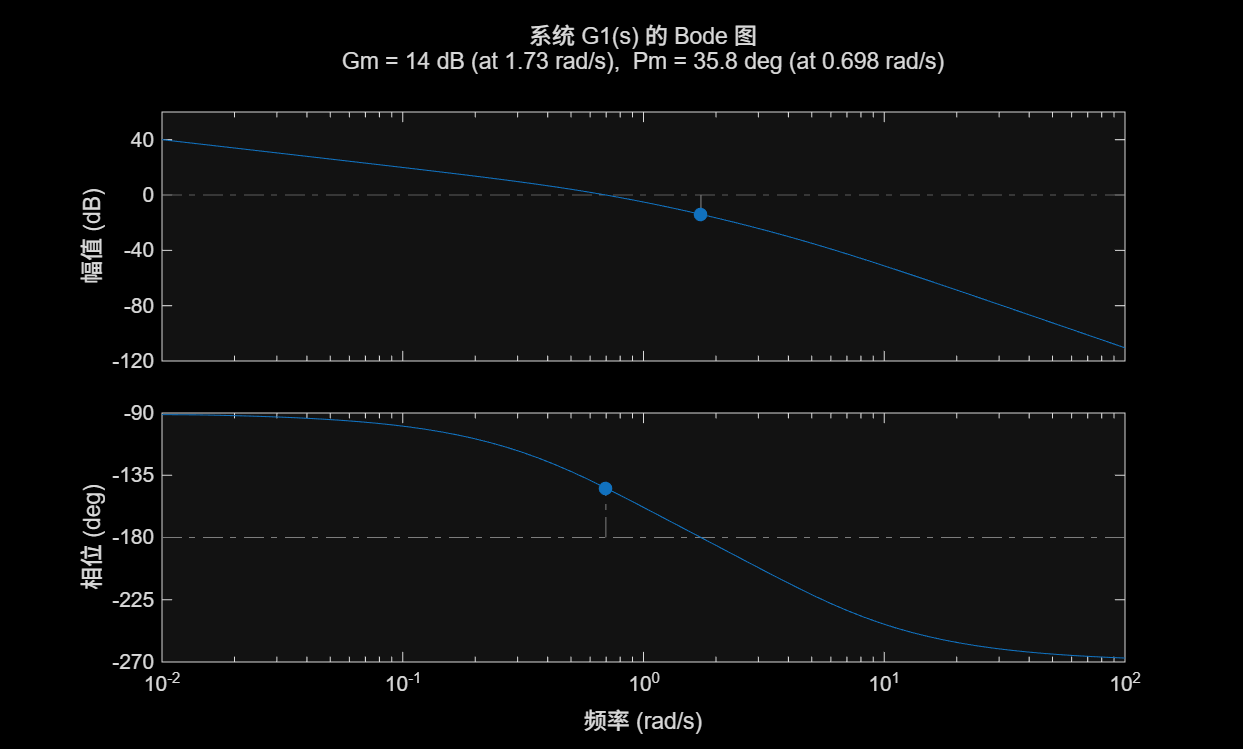
\includegraphics[width=0.80\textwidth]{./figures/Task01_Figure_01.png}
    \caption{系统G1(s)的Bode图}
    \label{fig:task01_fig1}
\end{figure}

\begin{figure}[H]
    \centering
    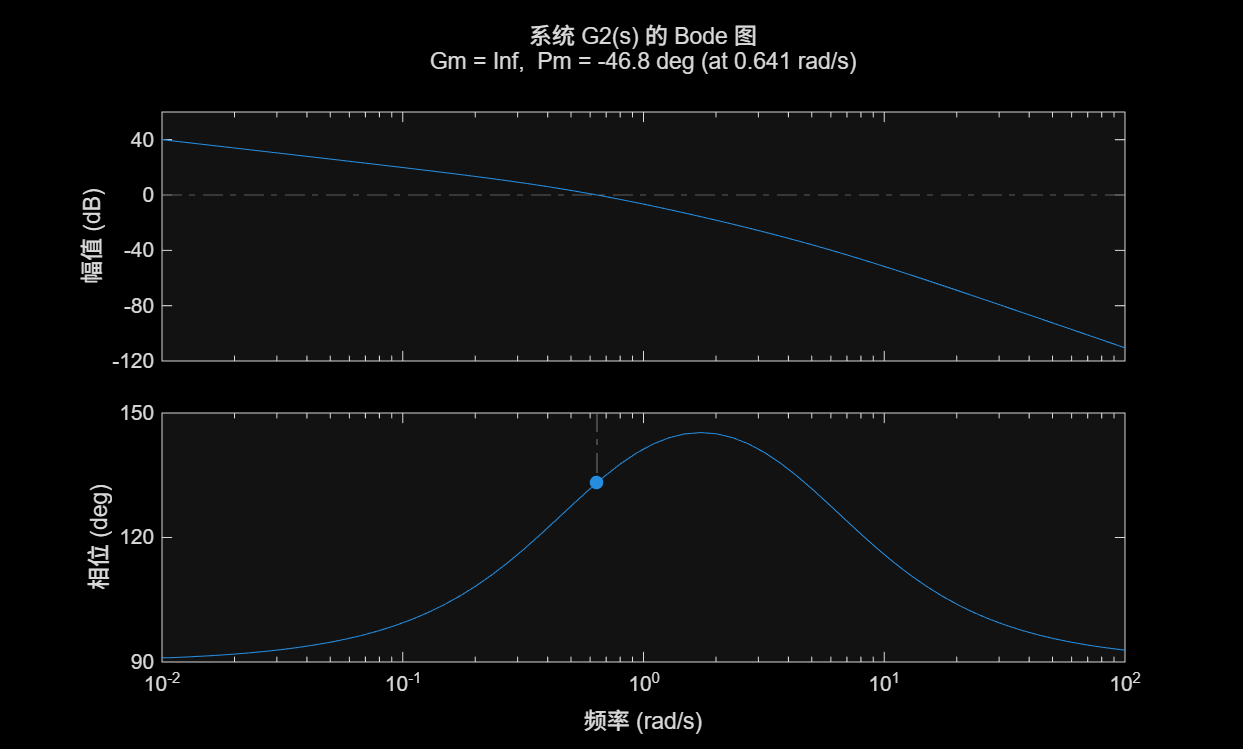
\includegraphics[width=0.80\textwidth]{./figures/Task01_Figure_02.png}
    \caption{系统G2(s)的Bode图}
    \label{fig:task01_fig2}
\end{figure}

Bode图分析结果如表~\ref{tab:task01_bode}~所示。

\begin{table}[H]
    \centering
    \caption{Bode图法稳定性分析结果}
    \label{tab:task01_bode}
    \begin{tabular}{cccc}
        \toprule
        系统 & 幅值裕度（dB） & 相角裕度（deg） & 稳定性结论 \\
        \midrule
        G1(s) & 13.98 & 35.77 & 闭环稳定 \\
        G2(s) & Inf & $-46.78$ & 闭环不稳定 \\
        \bottomrule
    \end{tabular}
\end{table}

G1(s)的幅值裕度为13.98~dB，相角裕度为35.77$^\circ$，均为正值，故闭环系统稳定。G2(s)的相角裕度为$-46.78^\circ$（负值），故闭环系统不稳定。该结果与通过开环传递函数中一次项系数符号的直接判断一致：G1(s)分母中$s$项系数$+3$表示系统稳定，G2(s)分母中$s$项系数$-3$（存在右半平面极点）表示系统不稳定。

\subsection{Task 02：系统能控性与能观性分析}

已知连续系统的传递函数模型：
\[
G(s) = \frac{s + a}{s^3 + 10s^2 + 27s + 8}
\]
当$a = -2, 0, +2$时，判别系统的能控性与能观性。

系统状态空间实现采用控制器标准型（companion form）：

\[
\boldsymbol{A} = \begin{bmatrix}
-10 & -27 & -8 \\
1 & 0 & 0 \\
0 & 1 & 0
\end{bmatrix},\quad
\boldsymbol{B} = \begin{bmatrix}
1 \\ 0 \\ 0
\end{bmatrix},\quad
\boldsymbol{C} = \begin{bmatrix}
0 & 1 & a
\end{bmatrix},\quad
D = 0
\]

系统极点为$-4.8315$、$-4.8315$、$-0.3369$，全部在左半平面，系统稳定。

\begin{figure}[H]
    \centering
    
\includegraphics[width=0.95\textwidth]{./figures/Task02_Figure_01.png}
    \caption{不同a值下的零极点图}
    \label{fig:task02_fig1}
\end{figure}

\begin{figure}[H]
    \centering
    
\includegraphics[width=0.95\textwidth]{./figures/Task02_Figure_02.png}
    \caption{不同a值下的阶跃响应对比}
    \label{fig:task02_fig2}
\end{figure}

\begin{figure}[H]
    \centering
    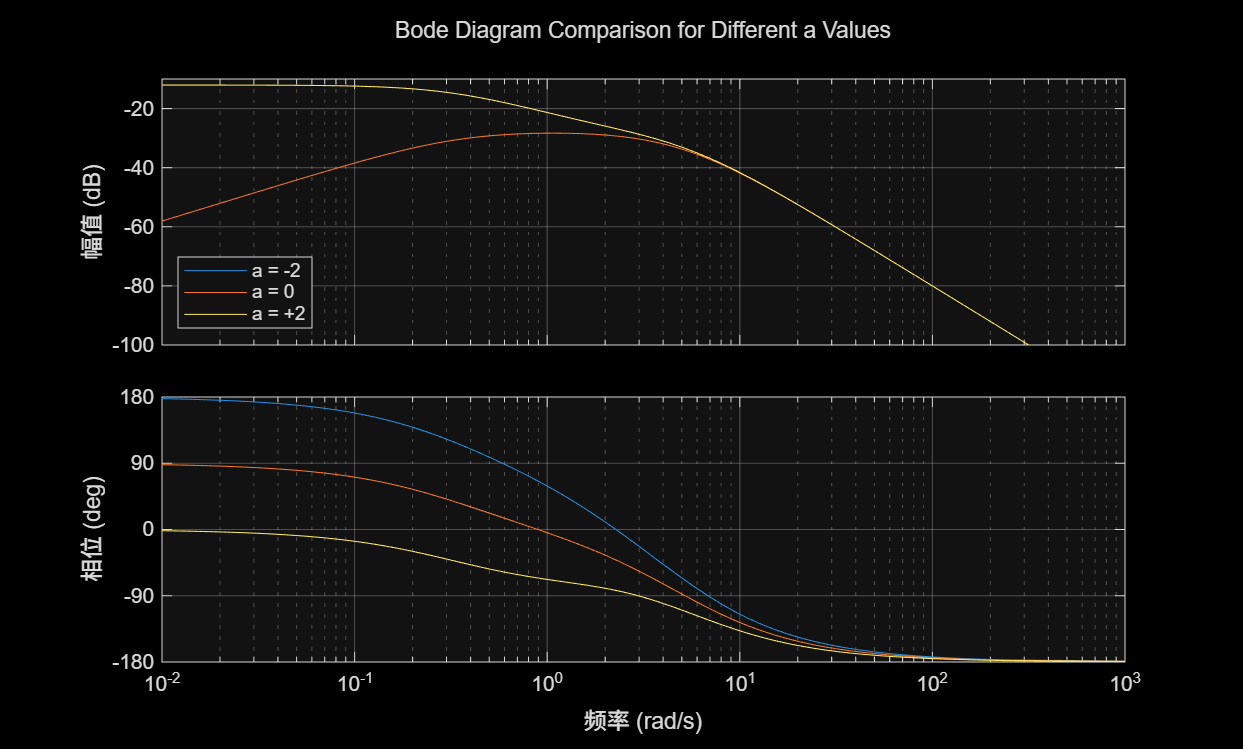
\includegraphics[width=0.95\textwidth]{./figures/Task02_Figure_03.png}
    \caption{不同a值下的Bode图对比}
    \label{fig:task02_fig3}
\end{figure}

\begin{table}[H]
    \centering
    \caption{能控性与能观性分析结果汇总}
    \label{tab:task02_results}
    \begin{tabular}{cccccc}
        \toprule
        $a$ & rank(Co) & rank(Ob) & 能控性（矩阵） & 能观性（矩阵） & Gramian验证 \\
        \midrule
        $-2$ & 3 & 3 & 完全能控 & 完全能观 & 一致 \\
        $0$  & 3 & 3 & 完全能控 & 完全能观 & 一致 \\
        $+2$ & 3 & 3 & 完全能控 & 完全能观 & 一致 \\
        \bottomrule
    \end{tabular}
\end{table}

能控性矩阵为：
\[
\boldsymbol{C}_o = [\boldsymbol{B}, \boldsymbol{AB}, \boldsymbol{A}^2\boldsymbol{B}] = \begin{bmatrix}
1 & -10 & 73 \\
0 & 1 & -10 \\
0 & 0 & 1
\end{bmatrix}
\]
$\text{rank}(\boldsymbol{C}_o) = 3 = n$，三种参数下系统均为完全能控。

能观性矩阵随$a$变化：
\[
\boldsymbol{O}_b(a=-2) = \begin{bmatrix}
0 & 1 & -2 \\
1 & -2 & 0 \\
-12 & -27 & -8
\end{bmatrix},\quad
\boldsymbol{O}_b(a=0) = \begin{bmatrix}
0 & 1 & 0 \\
1 & 0 & 0 \\
-10 & -27 & -8
\end{bmatrix},\quad
\boldsymbol{O}_b(a=+2) = \begin{bmatrix}
0 & 1 & 2 \\
1 & 2 & 0 \\
-8 & -27 & -8
\end{bmatrix}
\]
均满秩（$\text{rank}(\boldsymbol{O}_b) = 3$），三种参数下系统均为完全能观。

Gramian矩阵验证结果与能控性/能观性矩阵判据一致，均满足$\text{rank}(\boldsymbol{W}_c) = \text{rank}(\boldsymbol{W}_o) = 3$。

实验表明，参数$a$的变化影响零点的位置，从而影响系统的动态响应特性（如阶跃响应的初始值和稳态值），但不改变系统的能控性和能观性结构。

\subsection{Task 03：采样率对离散化的影响}

对Task 01中G2(s)的穿越频率进行分析，并用不同采样率将其离散化。
\[
G_2(s) = \frac{3}{s^3 + 5s^2 - 3s}
\]

增益穿越频率（Gain Crossover Frequency）：
\begin{itemize}
    \item $w_c = 0.641$~rad/s
    \item $f_1 = w_c/(2\pi) = 0.102$~Hz
\end{itemize}

采用零阶保持器（ZOH）方法，以$f = f_1$、$3f_1$、$10f_1$三种采样率将连续系统离散化，绘制Bode图和Nyquist图，并分析离散化精度。

\begin{figure}[H]
    \centering
    
\includegraphics[width=0.85\textwidth]{./figures/Task03_Figure_01.png}
    \caption{$f = f_1$（$T_s = 9.802$~s）时的Bode图和Nyquist图}
    \label{fig:task03_fig1}
\end{figure}

\begin{figure}[H]
    \centering
    
\includegraphics[width=0.85\textwidth]{./figures/Task03_Figure_02.png}
    \caption{$f = 3f_1$（$T_s = 3.267$~s）时的Bode图和Nyquist图}
    \label{fig:task03_fig2}
\end{figure}

\begin{figure}[H]
    \centering
    
\includegraphics[width=0.85\textwidth]{./figures/Task03_Figure_03.png}
    \caption{$f = 10f_1$（$T_s = 0.980$~s）时的Bode图和Nyquist图}
    \label{fig:task03_fig3}
\end{figure}

\begin{table}[H]
    \centering
    \caption{不同采样率下离散系统与连续系统的对比}
    \label{tab:task03_results}
    \small
    \begin{tabular}{cccccc}
        \toprule
        采样率 & $T_s$（s） & 幅值裕度（dB） & 相角裕度（deg） & 幅值误差（dB） & 相角误差（deg） \\
        \midrule
        连续 & N/A & Inf & $-46.78$ & --- & --- \\
        $f = f_1$ & 9.802 & Inf & Inf & 332.05 & 313.22 \\
        $f = 3f_1$ & 3.267 & Inf & $-109.75$ & 1.51 & 68.82 \\
        $f = 10f_1$ & 0.980 & Inf & $-64.90$ & 0.14 & 18.08 \\
        \bottomrule
    \end{tabular}
\end{table}

\textbf{结果分析：}
\begin{enumerate}
    \item \textbf{$f = f_1$（最低采样率）：}采样频率等于穿越频率，Nyquist频率（0.05~Hz）低于信号频率成分，严重违反香农采样定理。离散系统完全失真，幅值误差高达332.05~dB，频率响应无法反映连续系统的特性。
    \item \textbf{$f = 3f_1$：}Nyquist频率（0.15~Hz）超过穿越频率，满足基本Nyquist准则。但离散化精度仍有限，幅值误差1.51~dB，相角误差68.82$^\circ$，低频段匹配尚可。
    \item \textbf{$f = 10f_1$：}高采样率下离散系统与连续系统的频率响应高度吻合，幅值误差仅0.14~dB，相角误差18.08$^\circ$。零阶保持器引入的相位滞后在感兴趣的频率范围内影响较小。
\end{enumerate}

\textbf{结论：}采样率越高，离散系统越精确地逼近连续系统的频率响应。建议在实际数字控制系统实现中，采样率至少取系统穿越频率的10倍，以保证足够的离散化精度和控制性能。

\section{实验总结}
本次实验围绕控制系统现代分析方法，系统地进行了稳定性分析、能控性能观性分析以及采样率影响分析三个方面的实践。

\textbf{稳定性分析方面：}
\begin{enumerate}
    \item 通过代数法（Routh判据和求特征根）和频域法（Bode图）两种方法对系统进行稳定性判别，两种方法结论一致，验证了代数判据与频域判据的等价性。
    \item 对于G1(s)$= 3/(s^3 + 5s^2 + 3s)$，幅值裕度13.98~dB、相角裕度35.77$^\circ$，系统稳定；对于G2(s)$= 3/(s^3 + 5s^2 - 3s)$，相角裕度$-46.78^\circ$，系统不稳定。G2(s)的不稳定性源于其开环传递函数包含一个右半平面极点（$s$项系数为$-3$）。
\end{enumerate}

\textbf{能控性与能观性分析方面：}
\begin{enumerate}
    \item 对传递函数$G(s) = (s + a)/(s^3 + 10s^2 + 27s + 8)$在$a = -2, 0, +2$三种参数下进行了分析，能控性矩阵和能观性矩阵的秩均为3（满秩），Gramian矩阵验证一致。
    \item 三种参数下系统均为完全能控且完全能观。参数$a$的变化影响零点的位置和系统动态响应特性（阶跃响应、Bode图），但不改变能控性和能观性结构。
    \item 能控性矩阵与系统矩阵$\boldsymbol{A}$和输入矩阵$\boldsymbol{B}$有关，与输出矩阵$\boldsymbol{C}$（参数$a$所在位置）无关，因此参数$a$不影响能控性。而能观性矩阵虽与$\boldsymbol{C}$有关，但三种参数下均满秩，说明该系统的结构固有能观。
\end{enumerate}

\textbf{采样率影响分析方面：}
\begin{enumerate}
    \item 对不稳定系统G2(s)进行了从连续到离散的转换，研究了$f = f_1$、$3f_1$、$10f_1$三种采样率的影响。
    \item $f = f_1$时离散模型严重失真；$f = 3f_1$时精度有所改善但仍有较大相位误差；$f = 10f_1$时离散模型与连续模型高度吻合。
    \item 推荐实际应用中采样率至少取系统穿越频率的10倍，以保证数字控制系统的性能。
\end{enumerate}

本次实验加深了对控制系统稳定性、能控能观性以及数字离散化理论的理解，掌握了MATLAB控制系统工具箱在系统分析中的综合运用方法。

\section{实验源码}

\subsection{Task 01：系统稳定性分析}
\begin{lstlisting}[language=Matlab]
% 系统稳定性分析
clc;
clear;
close all;
diary('results/logs/Task01_output.log');

%% 1.1 代数法稳定性判据
% 已知开环传递函数 G(s) = 100*(s+3) / [s(s+1)(s+10)]
% 闭环特征多项式 = 1 + G(s) = 0

% 开环分母展开
den_open = conv([1 0], conv([1 1], [1 10]));
num_open = 100 * [1 3];

% 将分子补零到与分母相同长度
n_den = length(den_open);
n_num = length(num_open);
num_open = [zeros(1, n_den - n_num), num_open];

% 闭环特征多项式 = 分母 + 分子
den_closed = den_open + num_open;

% 方法一: 求分母多项式的根
roots_closed = roots(den_closed);
disp('=== 代数法稳定性判据 ===');
disp('方法一：求分母多项式的根');
disp(roots_closed);

% 判断稳定性
if all(real(roots_closed) < 0)
    disp('结论：闭环系统稳定');
else
    disp('结论：闭环系统不稳定');
end

% 方法二: Routh 判据
r = routh(den_closed, 1e-6);
disp('方法二：Routh 函数');
disp('Routh 表：');
disp(r);
disp('Routh 表第一列：');
disp(r(:, 1));

% 检查第一列是否有符号变化
first_col = r(:, 1);
sign_changes = 0;
for i = 1:length(first_col) - 1
    if first_col(i) * first_col(i + 1) < 0
        sign_changes = sign_changes + 1;
    end
end
fprintf('Routh 表第一列符号变化次数：%d\n', sign_changes);
if sign_changes == 0 && all(first_col > 0)
    fprintf('结论：闭环系统稳定\n');
else
    fprintf('结论：闭环系统不稳定，有 %d 个右半平面极点\n', sign_changes);
end

%% 1.2 Bode图法判断系统稳定性
% 两个单位负反馈系统的开环传递函数

% G1(s) = 3 / (s^3 + 5s^2 + 3s)
den_G1 = [1 5 3 0];
num_G1 = [3];

% G2(s) = 3 / (s^3 + 5s^2 - 3s)
den_G2 = [1 5 -3 0];
num_G2 = [3];

disp('========================================');
disp('=== Bode图法稳定性判据 ===');

% 绘制 G1 的 Bode 图
figure(1);
margin(tf(num_G1, den_G1));
title('系统 G1(s) 的 Bode 图');
saveas(gcf, 'results/figures/Task01_Figure_01.png');

[Gm1, Pm1, Wcg1, Wcp1] = margin(tf(num_G1, den_G1));
fprintf('\nG1(s): 幅值裕度 = %.2f dB, 相角裕度 = %.2f deg\n', ...
    20*log10(Gm1), Pm1);

if Pm1 > 0 && Gm1 > 1
    fprintf('结论：G1(s) 闭环系统稳定。\n');
else
    fprintf('结论：G1(s) 闭环系统不稳定。\n');
end

% 绘制 G2 的 Bode 图
figure(2);
margin(tf(num_G2, den_G2));
title('系统 G2(s) 的 Bode 图');
saveas(gcf, 'results/figures/Task01_Figure_02.png');

[Gm2, Pm2, Wcg2, Wcp2] = margin(tf(num_G2, den_G2));
fprintf('\nG2(s): 幅值裕度 = %.2f dB, 相角裕度 = %.2f deg\n', ...
    20*log10(Gm2), Pm2);

if Pm2 > 0 && Gm2 > 1
    fprintf('结论：G2(s) 闭环系统稳定。\n');
else
    fprintf('结论：G2(s) 闭环系统不稳定。\n');
end

diary off;
disp('Task 1 完成。');
\end{lstlisting}

\begin{lstlisting}[language=Matlab, caption={Routh判据辅助函数}]
function ra = routh(poli, epsilon)
% Routh-Hurwitz 稳定性判据数组计算
%   poli: 多项式系数向量（降幂排列）
%   epsilon: 行首零元素的替代值

dim = size(poli);
coeff = dim(2);
ra = zeros(coeff, ceil(coeff / 2));

% 组装第 1 行和第 2 行
for i = 1 : coeff
    ra(2 - rem(i, 2), ceil(i / 2)) = poli(i);
end

rows = coeff - 2;
index = zeros(rows, 1);

% 从底部到顶部形成索引向量
for i = 1 : rows
    index(rows - i + 1) = ceil(i / 2);
end

% 从第 3 行到最后一行
for i = 3 : coeff
    if all(ra(i - 1, :) == 0)   % 整行全为零
        a = coeff - i + 2;
        b = ceil(a / 2) - rem(a, 2) + 1;
        temp1 = ra(i - 2, 1 : b);
        temp2 = a : -2 : 0;
        ra(i - 1, 1 : b) = temp1 .* temp2;
    elseif ra(i - 1, 1) == 0    % 行首元素为零
        ra(i - 1, 1) = epsilon;
    end

    for j = 1 : index(i - 2)
        ra(i, j) = -det([ra(i - 2, 1), ra(i - 2, j + 1); ...
            ra(i - 1, 1), ra(i - 1, j + 1)]) / ra(i - 1, 1);
    end
end
end
\end{lstlisting}

\subsection{Task 02：系统能控性与能观性分析}
\begin{lstlisting}[language=Matlab]
% System Controllability and Observability Analysis
clc;
clear;
close all;
diary('results/logs/Task02_output.log');

fprintf('=================================================================\n');
fprintf('Task 2: System Controllability and Observability Analysis\n');
fprintf('Transfer function: G(s) = (s + a) / (s^3 + 10s^2 + 27s + 8)\n');
fprintf('a = -2, 0, +2\n');
fprintf('=================================================================\n\n');

a_values = [-2, 0, 2];
n = 3;  % system order

% Store results for summary
results_data = [];

for idx = 1:length(a_values)
    a = a_values(idx);
    fprintf('========== a = %d ==========\n', a);

    % Numerator and denominator
    num = [1, a];
    den = [1, 10, 27, 8];

    % Convert to state-space using tf2ss (controller canonical form)
    [A, B, C, D] = tf2ss(num, den);

    fprintf('State-space representation (controller canonical form):\n');
    fprintf('A =\n');
    disp(A);
    fprintf('B =\n');
    disp(B);
    fprintf('C =\n');
    disp(C);
    fprintf('D = %d\n', D);

    % --- Controllability Analysis ---
    Co = ctrb(A, B);
    rank_Co = rank(Co);
    fprintf('Controllability matrix Co =\n');
    disp(Co);
    fprintf('Rank(Co) = %d (system order n = %d)\n', rank_Co, n);

    if rank_Co == n
        fprintf('>> System is CONTROLLABLE.\n');
        controllable = true;
    else
        fprintf('>> System is NOT CONTROLLABLE.\n');
        controllable = false;
    end

    % --- Observability Analysis ---
    Ob = obsv(A, C);
    rank_Ob = rank(Ob);
    fprintf('\nObservability matrix Ob =\n');
    disp(Ob);
    fprintf('Rank(Ob) = %d (system order n = %d)\n', rank_Ob, n);

    if rank_Ob == n
        fprintf('>> System is OBSERVABLE.\n');
        observable = true;
    else
        fprintf('>> System is NOT OBSERVABLE.\n');
        observable = false;
    end

    % --- Verification using Gramians ---
    fprintf('\n--- Gramian Verification ---\n');
    sys = ss(A, B, C, D);
    poles = eig(A);
    fprintf('System poles: ');
    fprintf('%.4f  ', real(poles));
    fprintf('\n');

    if all(real(poles) < -1e-10)
        try
            Wc = gram(sys, 'c');
            Wo = gram(sys, 'o');
            fprintf('Controllability Gramian Wc =\n');
            disp(Wc);
            fprintf('Observability Gramian Wo =\n');
            disp(Wo);

            sv_Wc = svd(Wc);
            sv_Wo = svd(Wo);
            fprintf('Singular values of Wc: ');
            fprintf('%.6e  ', sv_Wc);
            fprintf('\n');
            fprintf('Singular values of Wo: ');
            fprintf('%.6e  ', sv_Wo);
            fprintf('\n');

            rank_Wc = rank(Wc, 1e-6);
            rank_Wo = rank(Wo, 1e-6);
            fprintf('Rank(Wc) = %d, Rank(Wo) = %d\n', rank_Wc, rank_Wo);

            if rank_Wc == n
                fprintf('Gramian verification: CONTROLLABLE.\n');
            else
                fprintf('Gramian verification: NOT CONTROLLABLE.\n');
            end
            if rank_Wo == n
                fprintf('Gramian verification: OBSERVABLE.\n');
            else
                fprintf('Gramian verification: NOT OBSERVABLE.\n');
            end
        catch ME
            fprintf('Gramian computation failed: %s\n', ME.message);
        end
    else
        fprintf('System has non-negative real poles; gramian skipped.\n');
    end

    results_data = [results_data; a, rank_Co, rank_Ob, ...
        controllable, observable];
    fprintf('\n');
end

% --- Summary Table ---
fprintf('=================================================================\n');
fprintf('SUMMARY OF RESULTS\n');
fprintf('=================================================================\n');
fprintf('  a   | rank(Co) | rank(Ob) | Controllable | Observable\n');
fprintf('------+----------+----------+--------------+------------\n');
for i = 1:size(results_data, 1)
    c_str = 'Yes';
    o_str = 'Yes';
    if results_data(i, 4) == 0
        c_str = 'No';
    end
    if results_data(i, 5) == 0
        o_str = 'No';
    end
    fprintf('  %2d  |    %d     |    %d     |     %s       |    %s\n', ...
        results_data(i, 1), results_data(i, 2), ...
        results_data(i, 3), c_str, o_str);
end
fprintf('=================================================================\n');
fprintf('Note: System order n = %d. Full rank (n) means controllable/observable.\n', n);
fprintf('=================================================================\n');

% --- Pole-Zero Maps ---
figure(1);
for idx = 1:length(a_values)
    a = a_values(idx);
    subplot(1, 3, idx);
    sys_tf = tf([1, a], [1, 10, 27, 8]);
    pzmap(sys_tf);
    title(sprintf('Pole-Zero Map (a = %d)', a));
    xlabel('Real Axis');
    ylabel('Imaginary Axis');
    grid on;
    [p, z] = pzmap(sys_tf);
    text_x = xlim;
    text_y = ylim;
    if ~isempty(z)
        text(text_x(1)+0.1*(text_x(2)-text_x(1)), ...
            text_y(2)-0.1*(text_y(2)-text_y(1)), ...
            sprintf('Zero: %.2f', real(z(1))), 'FontSize', 9);
    end
end
sgtitle('Pole-Zero Maps for Different a Values');
saveas(gcf, 'results/figures/Task02_Figure_01.png');

% --- Step Response Comparison ---
figure(2);
hold on;
colors = {'b', 'r', 'g'};
for idx = 1:length(a_values)
    a = a_values(idx);
    sys_tf = tf([1, a], [1, 10, 27, 8]);
    step(sys_tf, 10);
end
hold off;
title('Step Response Comparison');
xlabel('Time (seconds)');
ylabel('Amplitude');
legend('a = -2', 'a = 0', 'a = +2', 'Location', 'best');
grid on;
saveas(gcf, 'results/figures/Task02_Figure_02.png');

% --- Bode Diagram Comparison ---
figure(3);
hold on;
for idx = 1:length(a_values)
    a = a_values(idx);
    sys_tf = tf([1, a], [1, 10, 27, 8]);
    bode(sys_tf);
    hold on;
end
hold off;
title('Bode Diagram Comparison for Different a Values');
legend('a = -2', 'a = 0', 'a = +2', 'Location', 'southwest');
grid on;
saveas(gcf, 'results/figures/Task02_Figure_03.png');

fprintf('\nTask 2 completed successfully.\n');
diary off;
\end{lstlisting}

\subsection{Task 03：采样率对离散化的影响}
\begin{lstlisting}[language=Matlab]
% Sampling Rate Effects on Frequency Response Analysis
clc;
clear;
close all;
diary('results/logs/Task03_output.log');

fprintf('=================================================================\n');
fprintf('Task 3: Sampling Rate Effects on Frequency Response\n');
fprintf('=================================================================\n');

% G2(s) = 3 / (s^3 + 5s^2 - 3s)  (from Task 1, part 2)
num_G2 = [3];
den_G2 = [1, 5, -3, 0];
G2 = tf(num_G2, den_G2);

fprintf('Continuous system: G2(s) = 3/(s^3 + 5s^2 - 3s)\n\n');

% --- Find Gain Crossover Frequency ---
w_range = logspace(-3, 3, 10000);
[mag, ~, w_out] = bode(G2, w_range);
mag_dB = 20*log10(squeeze(mag));

% Find the 0 dB crossing (gain crossover frequency)
cross_idx = find(mag_dB(1:end-1) >= 0 & mag_dB(2:end) < 0, 1);
if isempty(cross_idx)
    cross_idx = find(mag_dB(1:end-1) <= 0 & mag_dB(2:end) > 0, 1);
end

if ~isempty(cross_idx)
    w1 = w_out(cross_idx);
    w2 = w_out(cross_idx + 1);
    m1 = mag_dB(cross_idx);
    m2 = mag_dB(cross_idx + 1);
    wc = w1 + (0 - m1) * (w2 - w1) / (m2 - m1);
else
    [~, min_idx] = min(abs(mag_dB));
    wc = w_out(min_idx);
    fprintf('Warning: No clear 0 dB crossing found. Using minimum magnitude frequency.\n');
end

f1 = wc / (2 * pi);
fprintf('Gain crossover frequency:\n');
fprintf('  wc = %.6f rad/s\n', wc);
fprintf('  f1 = %.6f Hz\n', f1);

% Also compute using margin function for comparison
[Gm_c, Pm_c, Wcg_c, Wcp_c] = margin(G2);
fprintf('\nMargin function results (continuous):\n');
fprintf('  Gain crossover freq (Wcp) = %.6f rad/s\n', Wcp_c);
fprintf('  Phase crossover freq (Wcg) = %.6f rad/s\n', Wcg_c);
fprintf('  Gain margin = %.2f dB\n', 20*log10(Gm_c));
fprintf('  Phase margin = %.2f deg\n', Pm_c);

% Use the margin function's crossover frequency if available
if ~isnan(Wcp_c) && Wcp_c > 0
    wc = Wcp_c;
    f1 = wc / (2 * pi);
    fprintf('\nUsing margin function crossover frequency: f1 = %.6f Hz\n', f1);
end

% --- Sampling Rates ---
fs_multipliers = [1, 3, 10];
num_rates = length(fs_multipliers);

w_bode = logspace(-2, 3, 800);

fprintf('\n=================================================================\n');
fprintf('Discretization and Analysis\n');
fprintf('=================================================================\n');

margin_results = zeros(num_rates, 4);

for i = 1:num_rates
    fs = fs_multipliers(i) * f1;
    Ts = 1 / fs;
    fn = fs / 2;
    wn = fn * 2 * pi;

    fprintf('\n--- Case %d: f = %d * f1 (Ts = %.6f s) ---\n', ...
        i, fs_multipliers(i), Ts);
    fprintf('  Sampling frequency fs = %.6f Hz\n', fs);
    fprintf('  Nyquist frequency fn = %.6f Hz (%.6f rad/s)\n', fn, wn);

    Gz = c2d(G2, Ts, 'zoh');
    fprintf('  Discrete transfer function Gz(z):\n');
    disp(Gz);

    figure(i);
    subplot(2, 1, 1);
    if fs_multipliers(i) <= 3
        w_display = logspace(-2, log10(wn * 1.2), 800);
        bode(G2, w_display);
        hold on;
        bode(Gz, w_display);
        hold off;
    else
        bode(G2, w_bode);
        hold on;
        bode(Gz, w_bode);
        hold off;
    end
    title(sprintf('Bode Diagram: f_s = %d * f_1 = %.4f Hz (T_s = %.6f s)', ...
        fs_multipliers(i), fs, Ts));
    legend('Continuous G2(s)', 'Discrete Gz(z)', ...
        'Location', 'southwest');
    grid on;

    subplot(2, 1, 2);
    nyquist(Gz);
    title(sprintf('Nyquist Diagram: Discrete System (f_s = %d * f_1)', fs_multipliers(i)));
    grid on;

    saveas(gcf, sprintf('results/figures/Task03_Figure_%02d.png', i));

    [Gm_d, Pm_d, Wcg_d, Wcp_d] = margin(Gz);

    fprintf('\n  Frequency Response Margins:\n');
    if ~isnan(Gm_d) && ~isnan(Pm_d)
        fprintf('  Gain margin (discrete) = %.2f dB\n', ...
            20*log10(Gm_d));
        fprintf('  Phase margin (discrete) = %.2f deg\n', Pm_d);
        margin_results(i, :) = [20*log10(Gm_d), Pm_d, Wcg_d, Wcp_d];
    else
        fprintf('  Margin computation returned NaN.\n');
        margin_results(i, :) = [NaN, NaN, NaN, NaN];
    end

    [mag_c, ph_c] = bode(G2, wc);
    [mag_d, ph_d] = bode(Gz, wc);
    fprintf('\n  Accuracy at crossover wc = %.4f rad/s:\n', wc);
    fprintf('  Continuous: |G(jwc)| = %.4f (%.2f dB), ', ...
        squeeze(mag_c), 20*log10(squeeze(mag_c)));
    fprintf('phase = %.2f deg\n', squeeze(ph_c));
    fprintf('  Discrete:   |Gz(e^{jwcTs})| = %.4f (%.2f dB), ', ...
        squeeze(mag_d), 20*log10(squeeze(mag_d)));
    fprintf('phase = %.2f deg\n', squeeze(ph_d));
    fprintf('  Magnitude error = %.4f dB\n', ...
        abs(20*log10(squeeze(mag_c)) - ...
        20*log10(squeeze(mag_d))));
    fprintf('  Phase error = %.4f deg\n', ...
        abs(squeeze(ph_c) - squeeze(ph_d)));
end

% --- Summary and Analysis ---
fprintf('\n=================================================================\n');
fprintf('SUMMARY: Sampling Rate Effects\n');
fprintf('=================================================================\n');
fprintf('  Sampling Rate  |  Ts (s)  |  Gain Margin (dB) | Phase Margin (deg)\n');
fprintf('----------------+----------+-------------------+--------------------\n');
fprintf('  Continuous     |   N/A    |      %.2f        |      %.2f\n', ...
    20*log10(Gm_c), Pm_c);
for i = 1:num_rates
    fprintf('  f = %d * f1    |  %.6f |      %.2f        |      %.2f\n', ...
        fs_multipliers(i), 1/(fs_multipliers(i)*f1), ...
        margin_results(i, 1), margin_results(i, 2));
end
fprintf('----------------+----------+-------------------+--------------------\n');

fprintf('\n--- Effect Analysis ---\n');
fprintf('1. At f = f1 (lowest sampling rate):\n');
fprintf('   - Sampling frequency equals crossover frequency.\n');
fprintf('   - Significant aliasing and distortion expected.\n');

fprintf('\n2. At f = 3*f1:\n');
fprintf('   - Nyquist frequency exceeds crossover frequency.\n');
fprintf('   - Basic Nyquist criterion satisfied.\n');

fprintf('\n3. At f = 10*f1:\n');
fprintf('   - High sampling rate provides good approximation.\n');
fprintf('   - Phase lag from ZOH is minimal.\n');

fprintf('\n--- Conclusion ---\n');
fprintf('Higher sampling rates yield more accurate frequency response matching.\n');
fprintf('A sampling rate of at least 10 times the crossover frequency is recommended\n');
fprintf('for accurate digital control system implementation.\n');

fprintf('\nTask 3 completed successfully.\n');
diary off;
\end{lstlisting}

\end{document}
